\section{Interpreter}

O padrão Interpreter define uma representação para 
a gramática de uma linguagem e um interpretador para 
interpretar sentenças dessa linguagem. Apesar da 
descrição generalista, o padrão 
pode ser utilizado para facilitar a resolução de 
problemas que ocorrem com frequência e que podem 
ser definidos através de uma árvore sintática 
abstrata.\cite{gamma:1995}

Esse padrão pode oferecer riscos quando a gramática 
é complexa. Como para cada regra será necessário 
definir uma nova classe, a hierarquia de classes 
resultante pode tornar-se muito grande e mais 
difícil de controlar. Em contrapartida, é 
fácil modificar ou estender a gramática, já 
que cada regra está encapsulada em uma classe 
diferente. A estrutura do padrão pode ser vista 
no diagrama da Figura \ref{interpreter_struct}.

\begin{figure}[htb]
	\caption{\label{interpreter_struct}Estrutura do Interpreter.}
	\begin{center}
	    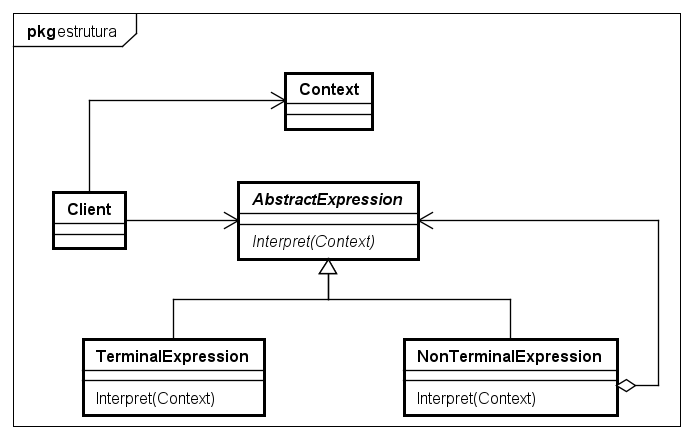
\includegraphics[scale=0.5]{5_padroes-contexto-funcional/5.3_comportamentais/5.3.03_interpreter/Interpreter_struct.png}
	\end{center}
\end{figure}

\subsection*{Exemplo Orientado a Objetos}

Como exemplo, o Interpreter pode ser utilizado para 
interpretar expressões booleanas. Cada classe definida 
representa uma expressão, que aceita constantes  
booleanas e operadores \textit{and}, \textit{or} e 
\textit{not}. No diagrama da Figura \ref{interpreter_exemplo}, 
as classes AndExpression, OrExpression e 
NotExpression representam operadores com subexpressões, 
enquanto a classe Constant representa um elemento 
terminal da expressão. A implementação do exemplo 
pode ser vista no Código \ref{oointerpreter}.

\begin{figure}[htb]
	\caption{\label{interpreter_exemplo}Exemplo de Interpreter.}
	\begin{center}
	    \includegraphics[scale=0.5]{5_padroes-contexto-funcional/5.3_comportamentais/5.3.03_interpreter/Interpreter_exemplo.png}
	\end{center}
\end{figure}

\begin{lstlisting}[caption={Interpreter Orientação a Objetos.},label=oointerpreter]

abstract class BooleanExpression {
  def Evaluate() : Boolean
}

class AndExpression(expression1 : BooleanExpression,
                    expression2 : BooleanExpression)
  extends BooleanExpression {
  override def Evaluate(): Boolean =
    expression1.Evaluate() && expression2.Evaluate()
}

class OrExpression(expression1 : BooleanExpression,
                   expression2 : BooleanExpression)
  extends BooleanExpression {
  override def Evaluate(): Boolean =
    expression1.Evaluate() || expression2.Evaluate()
}

class NotExpression(expression: BooleanExpression)
  extends BooleanExpression {
  override def Evaluate(): Boolean =
    !expression.Evaluate()
}

class Constant(value : Boolean)
  extends BooleanExpression {
  override def Evaluate(): Boolean = value
}
    
\end{lstlisting}

\subsection*{Contexto Funcional}

O padrão Interpreter pode ser refeito substituindo 
cada classe que representa uma regra da gramática 
por uma função de alta ordem. Essa função retorna a 
operação que realiza a interpretação. No Código 
\ref{fpinterpreter}, a operação de interpretação 
é definida pelo tipo Expression, na linha 2, como 
uma função que não recebe parâmetros e retorna um 
valor booleano. Na linha 4 é definida a regra para 
constantes, representada por uma função que recebe 
um valor booleano e retorna uma função que retorna 
esse mesmo valor.

Nas linhas 6 e 10 são definidas as funções 
AndExpression e OrExpression, ambas expressões 
binárias que recebem duas expressões e realizam 
uma operação. Por fim, a linha 14 define a função 
NotExpression, uma expressão unária que recebe 
apenas uma outra expressão como parâmetro e 
aplica uma função \textit{not} à mesma.

\begin{lstlisting}[caption={Interpreter Funcional.},label=fpinterpreter]
    
type Expression = () => Boolean

def Constant(value : Boolean) : Expression = () => value
  
def AndExpression(expression1 : Expression,
                  expression2 : Expression) : Expression =
  () => expression1() && expression2()
  
def OrExpression(expression1 : Expression,
                 expression2 : Expression) : Expression =
  () => expression1() || expression2()
  
def NotExpression(expression: Expression) : Expression =
  () => !expression()
    
\end{lstlisting}

A vantagem da implementação funcional desse 
padrão é demonstrada no Código \ref{fpinterpreter2}, 
onde é possível aproveitar as funções de alta 
ordem para definir operadores binários e unários 
genéricos. Eles são definidos na linha 2 pela função 
BinaryExpression e na linha 8 pela função 
UnaryExpression. Nas linhas 13, 18 e 23, são 
definidas funções equivalentes às funçãos 
AndExpression, OrExpression e NotExpression do 
Código \ref{fpinterpreter}.

\begin{lstlisting}[caption={Interpreter com regras genéricas.},label=fpinterpreter2]
    
def BinaryExpression(expression1 : Expression,
  expression2 : Expression,
  function : (Boolean, Boolean) => Boolean)
: Expression =
() => function(expression1(), expression2())

def UnaryExpression(expression: Expression,
  function : (Boolean) => Boolean) 
: Expression =
() => function(expression())

val andExpression = (expression1 : Expression, 
   expression2 : Expression) =>
BinaryExpression(expression1, expression2, 
 (e1 : Boolean, e2 : Boolean) => e1 && e2)

val orExpression = (expression1 : Expression, 
  expression2 : Expression) =>
BinaryExpression(expression1, expression2, 
  (e1 : Boolean, e2 : Boolean) => e1 || e2)

val notExpression = (expression : Expression) =>
  UnaryExpression(expression, (e : Boolean) => !e)
    
\end{lstlisting}